\documentclass[12pt, 
hyperref={colorlinks=true, linkcolor=blue, urlcolor=cyan},dvipsnames]{beamer}
\usetheme{default} 

\setbeamertemplate{navigation symbols}{} %gets rid of navigation symbols
\setbeamertemplate{footline}{} %gets rid of bottom navigation bars
\setbeamertemplate{footline}[page number]{} %use this for page numbers

\setbeamertemplate{itemize items}[circle] %round bullet points
\setlength\parskip{10pt} % white space between paragraphs

\usepackage{wrapfig}
\usepackage{subfig}
\usepackage{setspace}
\usepackage{enumerate}
\usepackage{graphicx}
\usepackage{amsmath}
\usepackage{amsfonts}
\usepackage{amssymb}
\usepackage{amsthm}
\usepackage[UKenglish]{isodate}
\usepackage{verbatim}
\usepackage{xcolor}
\cleanlookdateon

% new amber color
\definecolor{amber}{rgb}{1.0, 0.75, 0.0}

\DeclareMathOperator{\argmin}{argmin}

% the preamble
\title{BIOST 311: \\ Regression Methods for the Health Sciences}
\author{Kelsey Grinde and Brian Williamson}
\institute{UW Biostatistics}
\date{Spring 2018}

\begin{document}
% title slide
\begin{frame}
\titlepage\thispagestyle{empty}
\end{frame}

% make it 1.something
\setbeamertemplate{footline}{%
  \raisebox{5pt}{\makebox[\paperwidth]{\makebox[120pt]{\scriptsize Last updated \today}\hfill\makebox[20pt]{\scriptsize 3.\insertframenumber~~}}}}  \newcounter{chap3}{\value{1}}
\setcounter{framenumber}{\value{chap3}}

\begin{frame}
\frametitle{CHAPTER 3: SURVIVAL ANALYSIS}
By the end of Chapter 3, you should be able to: \vspace{-0.3cm}

\begin{itemize}
\item Determine if a variable has been \textcolor{BurntOrange}{right-censored}
\item Discuss the \textcolor{red}{drawbacks} of treating a right-censored variable as binary or continuous
\item \textbf{Interpret Kaplan-Meier curves}, and create them in \texttt{R}
\item \textbf{Implement and interpret} a log-rank test for equating survival curves
\item \textbf{Formulate a regression model} given a scientific or statistical question about a right-censored outcome
\item \textbf{Interpret the coefficients} for a (simple or multiple) proportional hazards regression model
\item \textbf{Interpret confidence intervals and p-values} for proportional hazards regression coefficients
\item Use \texttt{R} to fit a proportional hazards regression model and create figures/tables to support your regression analysis
\end{itemize}

\end{frame}

\section{Censored outcomes}
\begin{frame}
\frametitle{SECTION 1: CENSORED OUTCOMES}
Up to this point, we have focused on questions involving \textcolor{blue}{quantitative} or \textcolor{BurntOrange}{binary} outcomes: 
\begin{itemize}
\item Is lung function (\textcolor{blue}{FEV}) associated with smoking, after adjusting for age, height, and sex?
\item Is cognitive function (\textcolor{blue}{DSST score}) associated with alcohol use, adjusting for age, sex, and education?
\item Is \textcolor{BurntOrange}{diabetes} associated with BMI, after adjusting for sex?
\end{itemize}
\end{frame}

\begin{frame}
\frametitle{SECTION 1: CENSORED OUTCOMES}
However, we are often interested in scientific questions that involve \textcolor{blue}{time-to-event} outcomes:
\begin{itemize}
\item Is \textcolor{blue}{time to first seizure post operation to remove a brain tumor} associated with pre-operation case review by an epileptologist, in children with both epilepsy and brain tumor?
\item Is \textcolor{blue}{time to promotion for university faculty members} associated with sex?
\item Is \textcolor{blue}{time to death from any cause} associated with serum levels of C reactive protein?
\end{itemize}
\end{frame}

\begin{frame}
\frametitle{Characteristics of survival data}
{\fontsize{10pt}{7.2}\selectfont
Sample of the observed times until first severe panic attack (in weeks):
\hspace*{-1cm}\begin{tabular}{|c|c|c|c|c|c|c|c|c|c|}
\hline
\textcolor{blue}{meditation group} & 14.29 & 7.74 & 21 & 25.18 & 2.83 & 17.57 & 19.13 & 0.14  \\
\hline
control group & 21 & 3.94 & 7.77 & 6.54 & 24 & 12.55 & 21.29 & 3.58 \\
\hline
\end{tabular}
}

We wish to study whether \textcolor{blue}{meditation} prolongs the \textbf{time until a severe panic attack} in patients suffering from a panic disorder.

To address this question, we: \vspace{-0.3cm}
\begin{itemize}
\item recruit 200 patients and randomize them to meditation or placebo;
\item follow each patient until their first severe panic attach post recruitment;
\item and compare the mean time until a severe panic attack in each group with a t-test
\end{itemize}

\end{frame}

\begin{frame}
\frametitle{Characteristics of survival data}
\centering
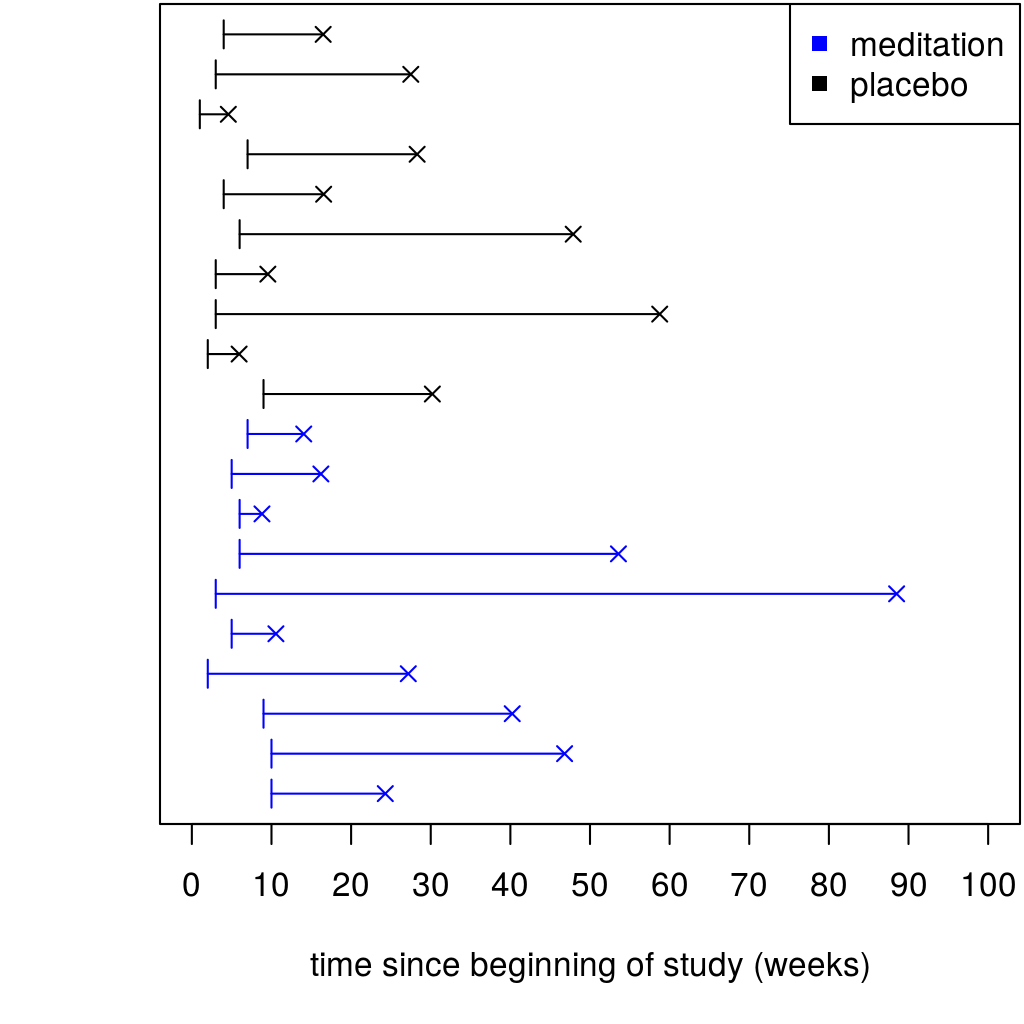
\includegraphics[width=0.8\textwidth]{figs/meditation_observed_study_time.png}
\end{frame}

\begin{frame}
\frametitle{Characteristics of survival data}
\centering
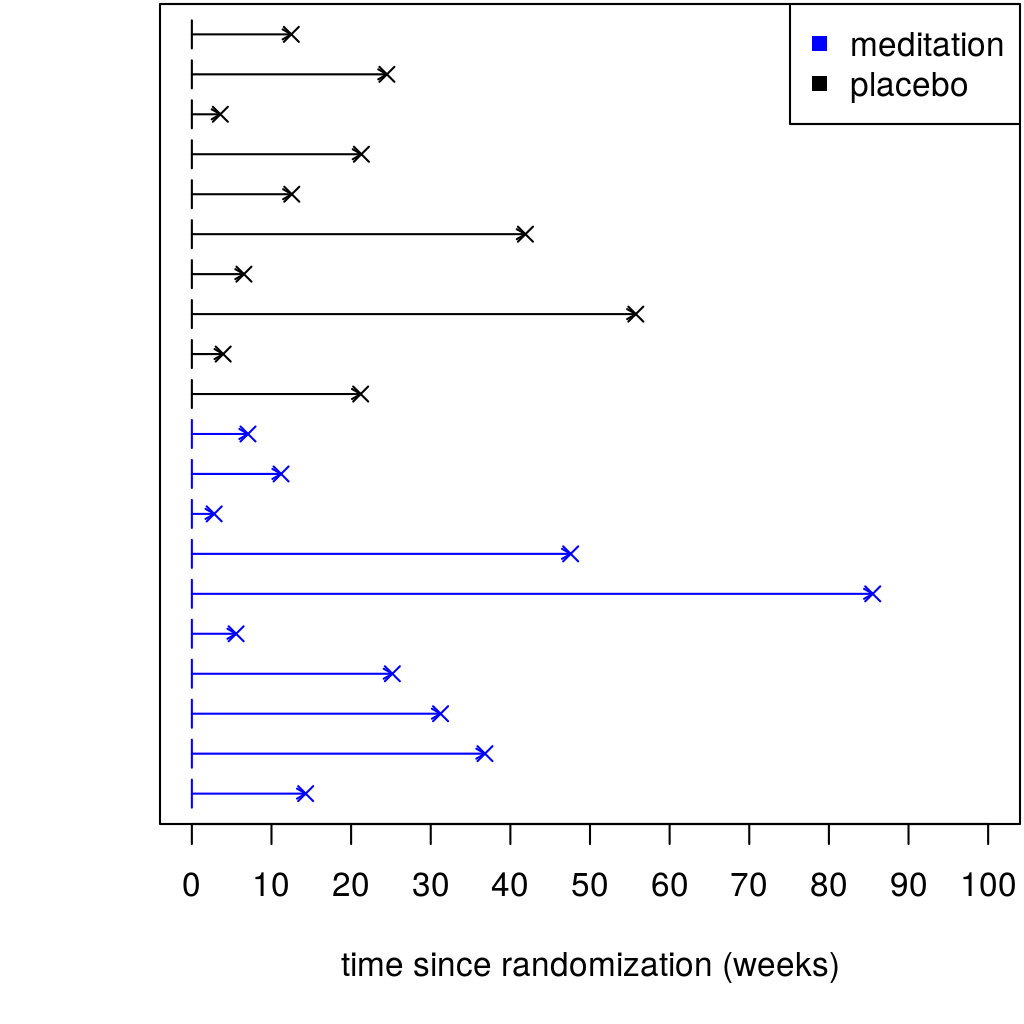
\includegraphics[width=0.8\textwidth]{figs/meditation_observed_rand_time.png}
\end{frame}

\begin{frame}
\frametitle{Characteristics of survival data}
In this hypothetical study, we were able to record the actual occurrence time \textcolor{blue}{for each participant}.

Is this typical of human studies? \pause \textcolor{red}{No!}

Why? \pause Some common reasons are:
\begin{itemize}
\item the study ended (e.g., after 30 weeks) and some participants had not yet had a severe panic attack (\textbf{administrative censoring})
\item the participant left the study before having had a severe panic attack (\textbf{loss to follow-up})
\end{itemize}

These all lead to \textbf{right-censored} data, where rather than knowing the value exactly, we know that the value exceeds some cutoff.
\end{frame}

\begin{frame}
\frametitle{Characteristics of survival data}
\centering
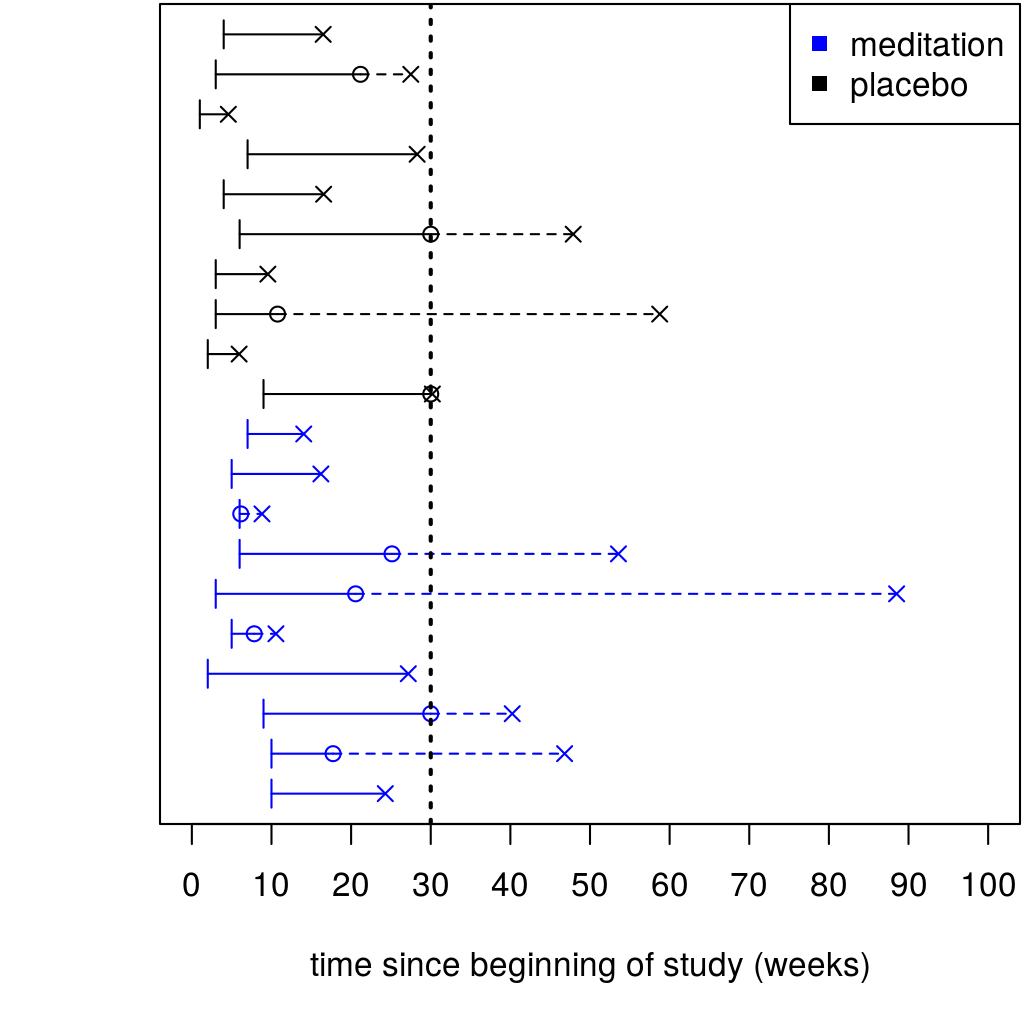
\includegraphics[width=0.8\textwidth]{figs/meditation_censored_study_time.png}
\end{frame}

\begin{frame}
\frametitle{Characteristics of survival data}
\centering
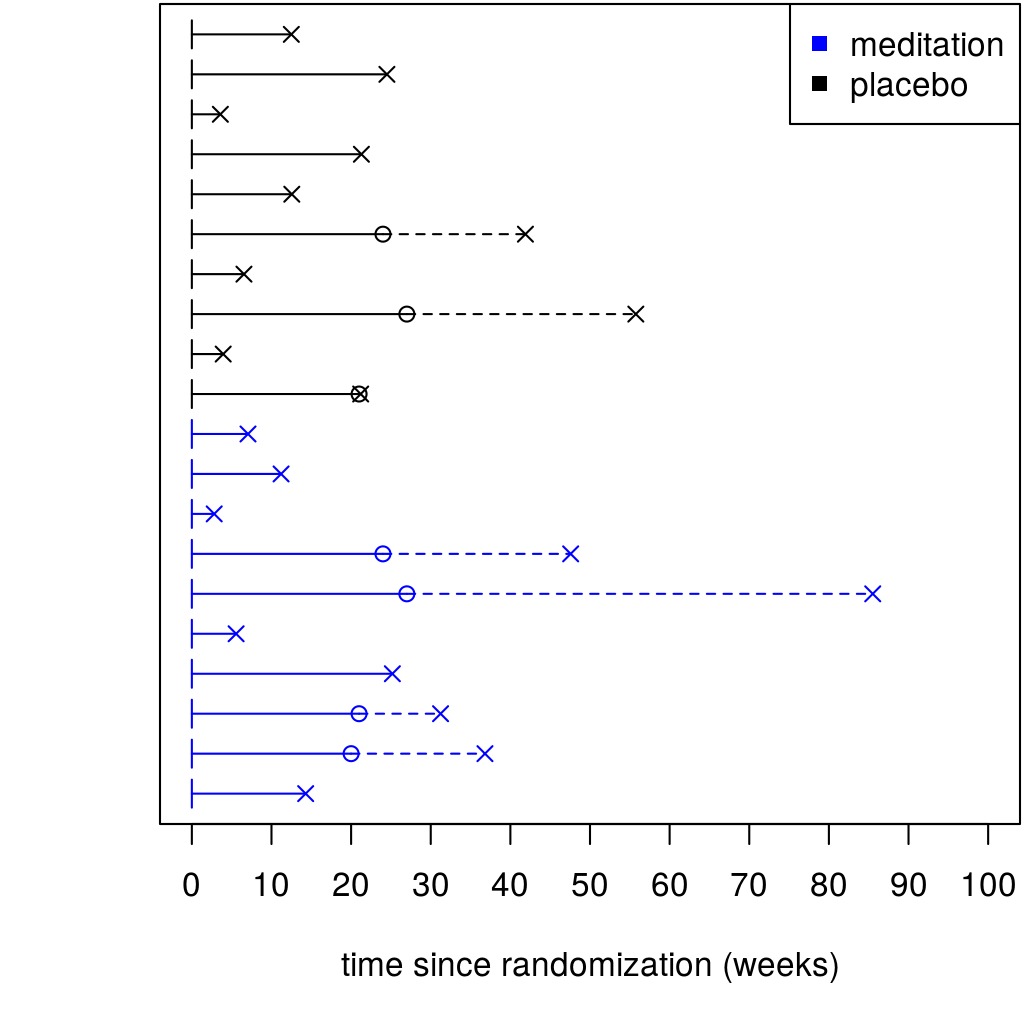
\includegraphics[width=0.8\textwidth]{figs/meditation_censored_rand_time.png}
\end{frame}

\begin{frame}
\frametitle{Characteristics of survival data}
{\fontsize{10pt}{7.2}\selectfont
The data can be represented as:
\hspace*{-1cm}\begin{tabular}{|c|c|c|c|c|c|c|c|c|c|}
\hline
\textcolor{blue}{meditation group} & 14.29  & \textcolor{red}{7.74+} & \textcolor{red}{21.00+} & 25.18  &  \textcolor{red}{2.83+} & \textcolor{red}{17.57+} & \textcolor{red}{19.13+} &  \textcolor{red}{0.14+}  \\
\hline
control group & \textcolor{red}{21.00+} &  \textcolor{red}{3.94+} &  \textcolor{red}{7.77+} &  6.54  & \textcolor{red}{24.00+} & 12.55  & 21.29 &  3.58 \\
\hline
\end{tabular}
}

\vspace{-0.6cm}
{\small
Should we treat these incompletely observed times as missing data? Should we throw them out? \pause \textcolor{red}{Either of these is a bad idea!} \vspace{-0.3cm}

\begin{itemize}
\item These observations contain valuable information:
{\scriptsize
\begin{itemize}
\item \textcolor{red}{20+}: the participant did not experience a severe panic attack before 20 weeks
\item their actual time until the first severe panic attack must be in the interval $(20, +\infty)$
\end{itemize}
}
\item These participants are not representative of the whole study population: valid estimation and inference when excluding missing data (which we have done so far) assumes that the people excluded are ``similar to'' the people still in the data (\textbf{missing completely at random})
\end{itemize}
}
\end{frame}

\begin{frame}
\frametitle{Characteristics of survival data}
Close or put away your notes and laptops. Then answer the following questions, paying attention your thought process (you will hand in your responses):
\begin{enumerate}
\item Are those with smaller or larger times more likely to be censored? Why?
\item Systematically excluding censored times could lead to \textcolor{red}{biased estimates}. Would this lead to an overestimation or an underestimation of the mean time until severe panic attack? Why?
\end{enumerate}

\end{frame}

\begin{frame}
\frametitle{Characteristics of survival data}
\begin{enumerate}
\item Are those with smaller or larger times more likely to be censored? Why?
\item[] \textcolor{blue}{Those with \textbf{larger times} are more likely to be censored; we only get to observe these people for a comparatively small amount of time, so we may miss their event}
\item Systematically excluding censored times could lead to \textcolor{red}{biased estimates}. Would this lead to an overestimation or an underestimation of the mean time until severe panic attack? Why?
\item[] \textcolor{blue}{\textbf{Underestimation}: if we exclude censored times, then we are effectively excluding these people with potentially longer times, and losing all of this information!}
\end{enumerate}

\end{frame}

\begin{frame}
\frametitle{Characteristics of survival data}
Sampling distribution of times in participants who become censored or uncensored, and the overall target population:\vspace{-0.4cm}
\begin{center}
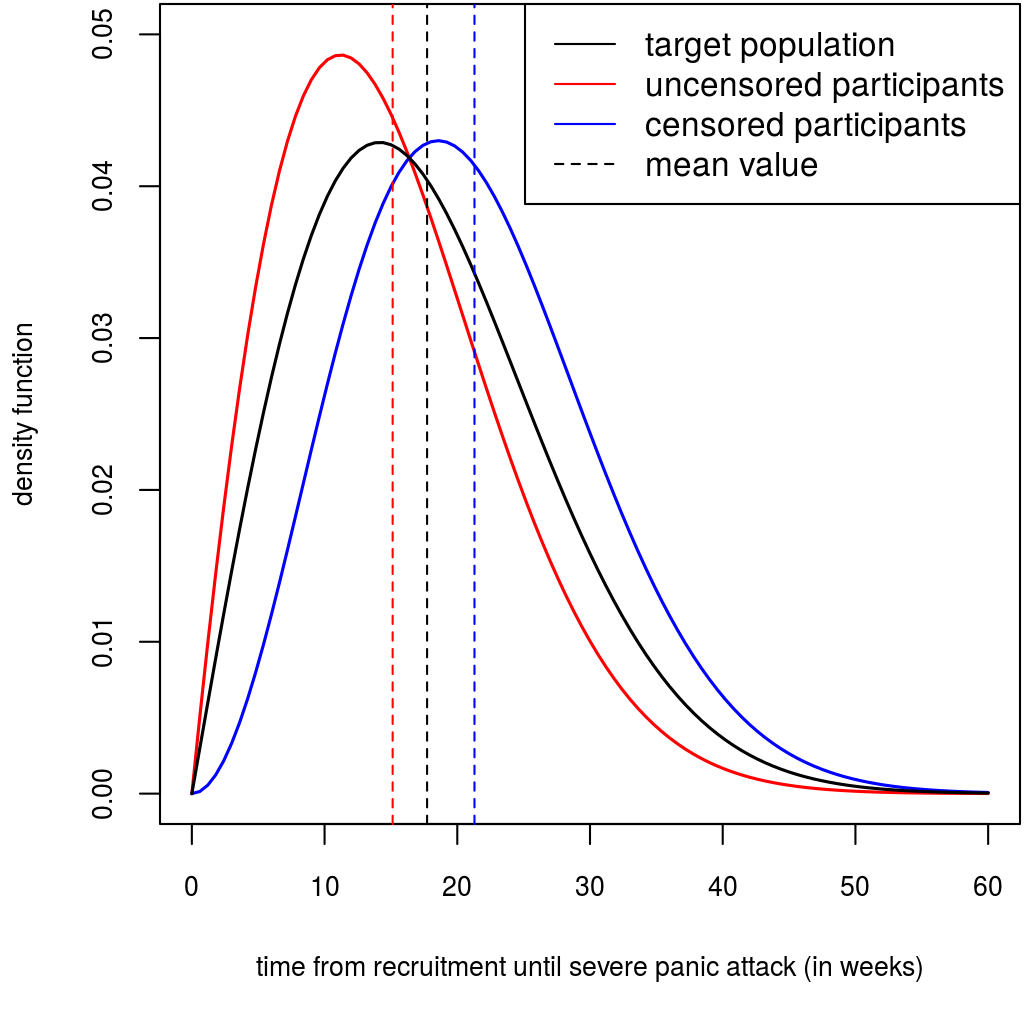
\includegraphics[height=0.8\textheight]{figs/meditation_density_versus_obs_time.png}
\end{center}
\end{frame}

\begin{frame}
\frametitle{Characteristics of survival data}
\textbf{Survival analysis} is the branch of statistics concerned with the analysis of \textbf{time-to-event data}.

Often, the goals of a survival analysis are to:
\begin{itemize}
\item describe the distribution of a time-to-event variable
\item compare the time-to-event distribution in different subpopulations
\item investigate the relationship between explanatory variables and the time-to-event distribution
\end{itemize}

Even when our time-to-event data do not truly mean survival (e.g., time to first severe panic attack), we still use the term ``survival''.
\end{frame}

\begin{frame}
\frametitle{Characteristics of survival data}
Why is time-to-event data special? Why can we not use standard methods? \vspace{-0.5cm}
\begin{itemize}
\item A time-to-event variable is positive and generally skewed
\item To appropriately define a time-to-event, we must specify:
{\scriptsize
\begin{itemize}
\item initiating event --- e.g., birth, recruitment into study, onset of disease
\item terminating event --- e.g., death, onset of disease
\item time scale --- e.g., calendar time, number of transfusions
\end{itemize}
}
\item Time-to-event data are generally observed subject to some incompleteness, of which \textbf{censoring} is a major type
\item Throwing away incomplete data generally results in
{\scriptsize
\begin{enumerate}
\item a loss of information (and increase in estimation uncertainty)
\item biased estimation procedures (most important!)
\end{enumerate}
}
\end{itemize}

\end{frame}

\begin{frame}
\frametitle{Characteristics of survival data}
A time-to-event variable is said to be \textbf{censored} if rather than being known exactly, it is known to lie in some set of values.

In this course, we will focus on \textbf{right censoring}, where we only know that the event occurred after the censoring point.

Right-censored data are the most common type of censored data found in applications!
\end{frame}

% risk set, plus movie
\begin{frame}
\frametitle{Characteristics of survival data}
Key concept: the \textbf{risk set}.

\textbf{Risk set at time $t$}: the collection of participants that \textcolor{blue}{could have experienced} their first severe panic attack at time $t$; in other words, those who were still at risk at time $t$.
\vspace{-0.3cm}
\begin{align*}
\textbf{fraction at risk at time } t = & \frac{\textbf{size of risk set at time } t}{\textbf{total sample size}}.
\end{align*}

A few observations:\vspace{-0.3cm}
\begin{itemize}
\item participants \textcolor{blue}{exit} the risk set either when they \textcolor{Aquamarine}{experience a severe panic attack} or when they \textcolor{red}{become right-censored}
\item with right-censored data, all participants are in the risk set at time 0 and the risk set necessarily shrinks over time
\item the \textcolor{blue}{size of the risk set} and the \textcolor{blue}{characteristics of its members} will be critical in survival analysis
\end{itemize}
\end{frame}

\begin{frame}
\frametitle{Characteristics of survival data}
\begin{center}
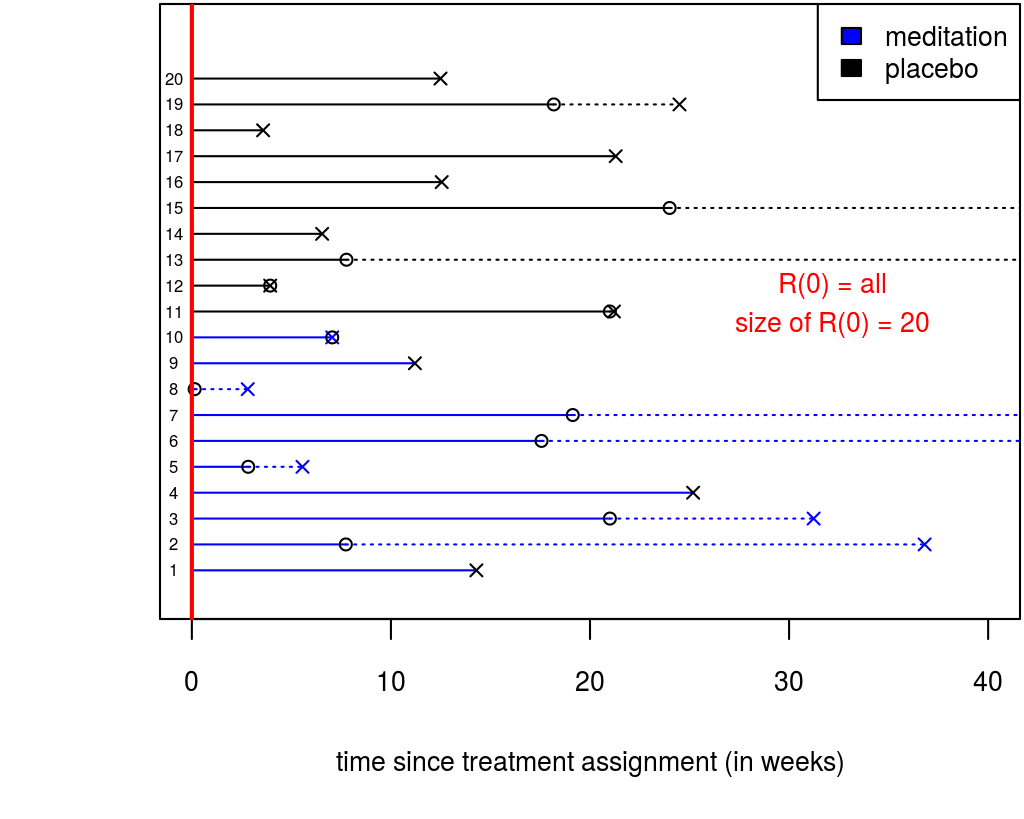
\includegraphics[height=0.8\textheight]{figs/risk_set_movie_0.png}
\end{center}
\end{frame}

\begin{frame}
\frametitle{Characteristics of survival data}
\begin{center}
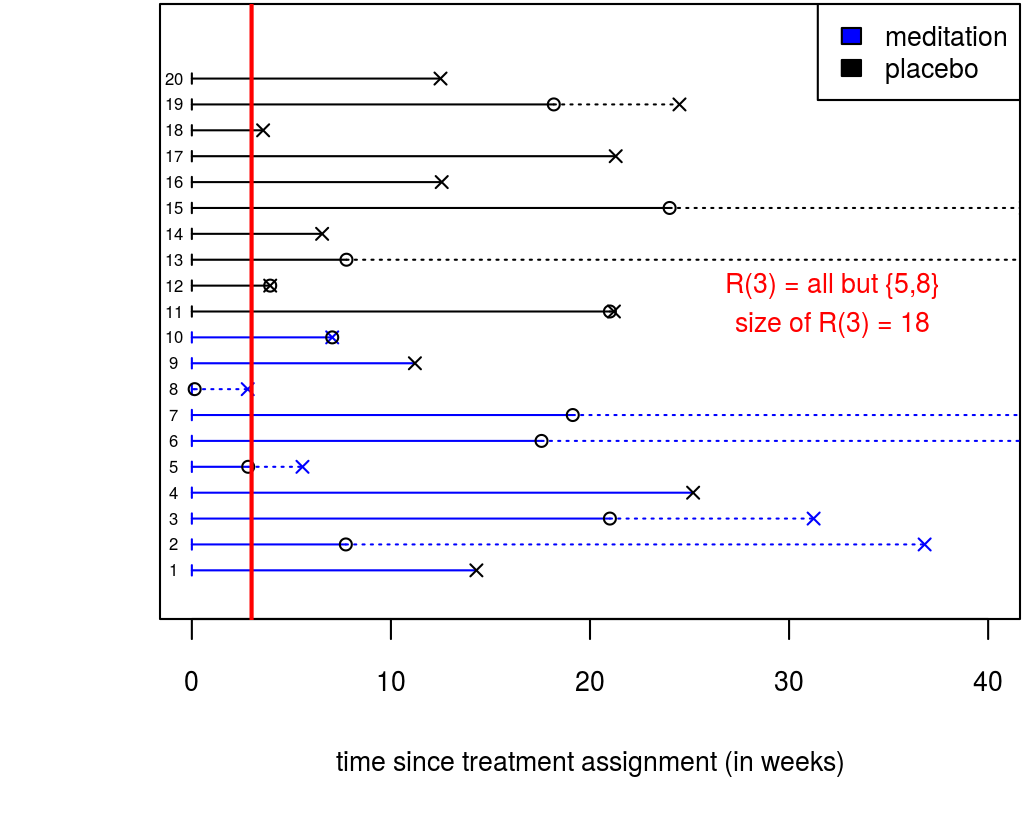
\includegraphics[height=0.8\textheight]{figs/risk_set_movie_1.png}
\end{center}
\end{frame}

\begin{frame}
\frametitle{Characteristics of survival data}
\begin{center}
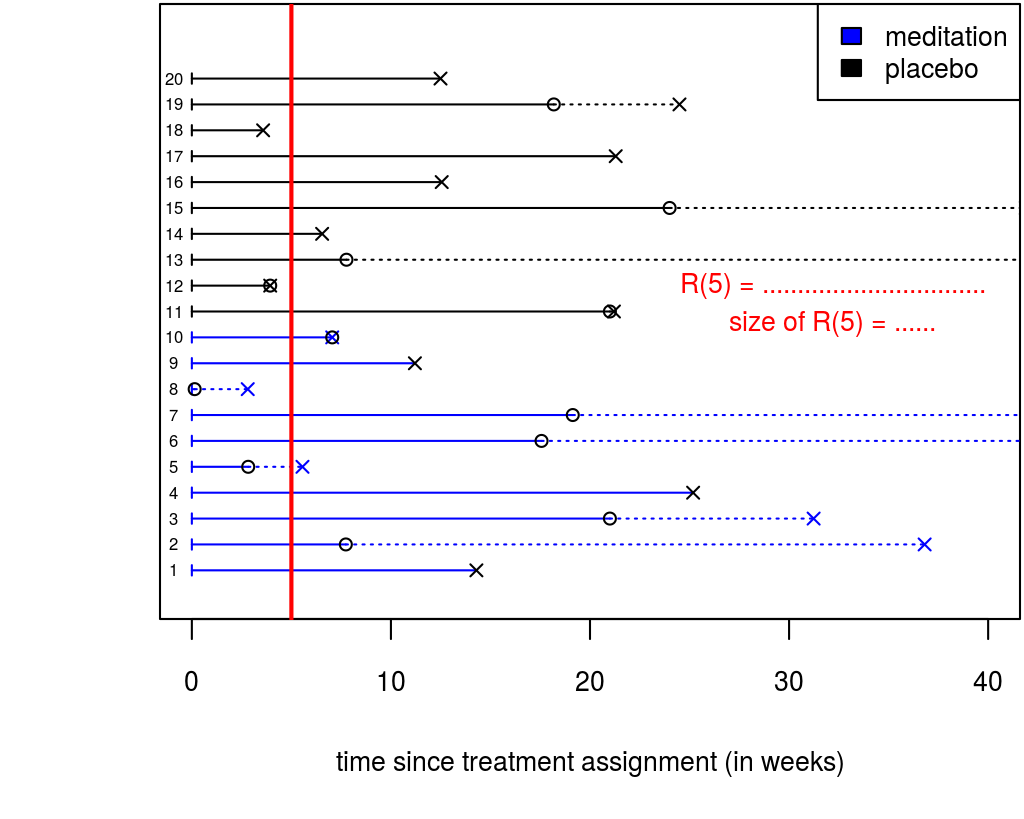
\includegraphics[height=0.8\textheight]{figs/risk_set_movie_2.png}
\end{center}
\end{frame}

\begin{frame}
\frametitle{Characteristics of survival data}
\begin{center}
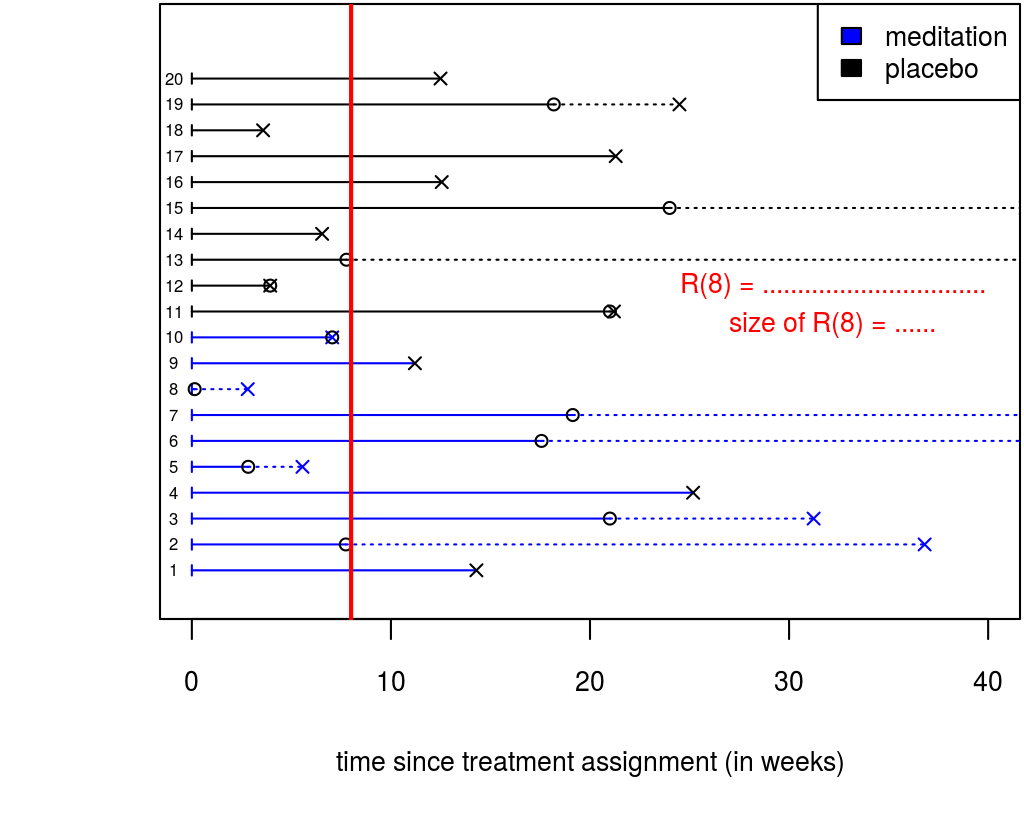
\includegraphics[height=0.8\textheight]{figs/risk_set_movie_3.png}
\end{center}
\end{frame}

\begin{frame}
\frametitle{Characteristics of survival data}
\begin{center}
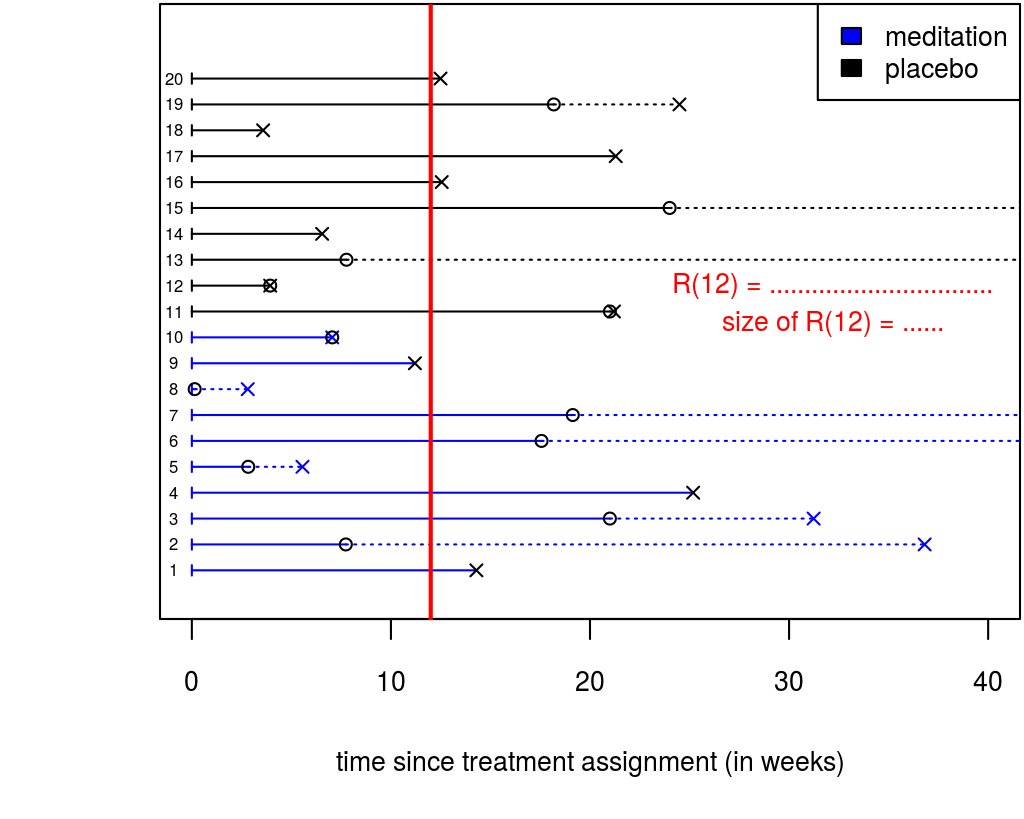
\includegraphics[height=0.8\textheight]{figs/risk_set_movie_4.png}
\end{center}
\end{frame}

\begin{frame}
\frametitle{Characteristics of survival data}
\begin{center}
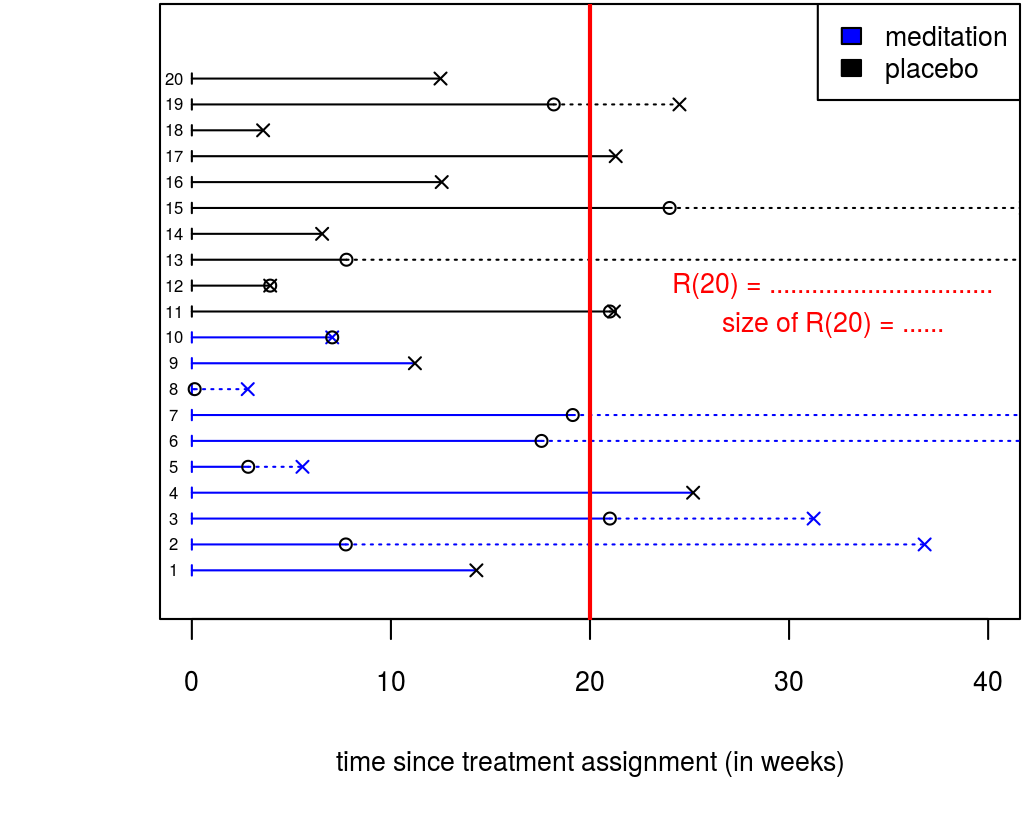
\includegraphics[height=0.8\textheight]{figs/risk_set_movie_5.png}
\end{center}
\end{frame}

\begin{frame}
\frametitle{Characteristics of survival data}
\begin{center}
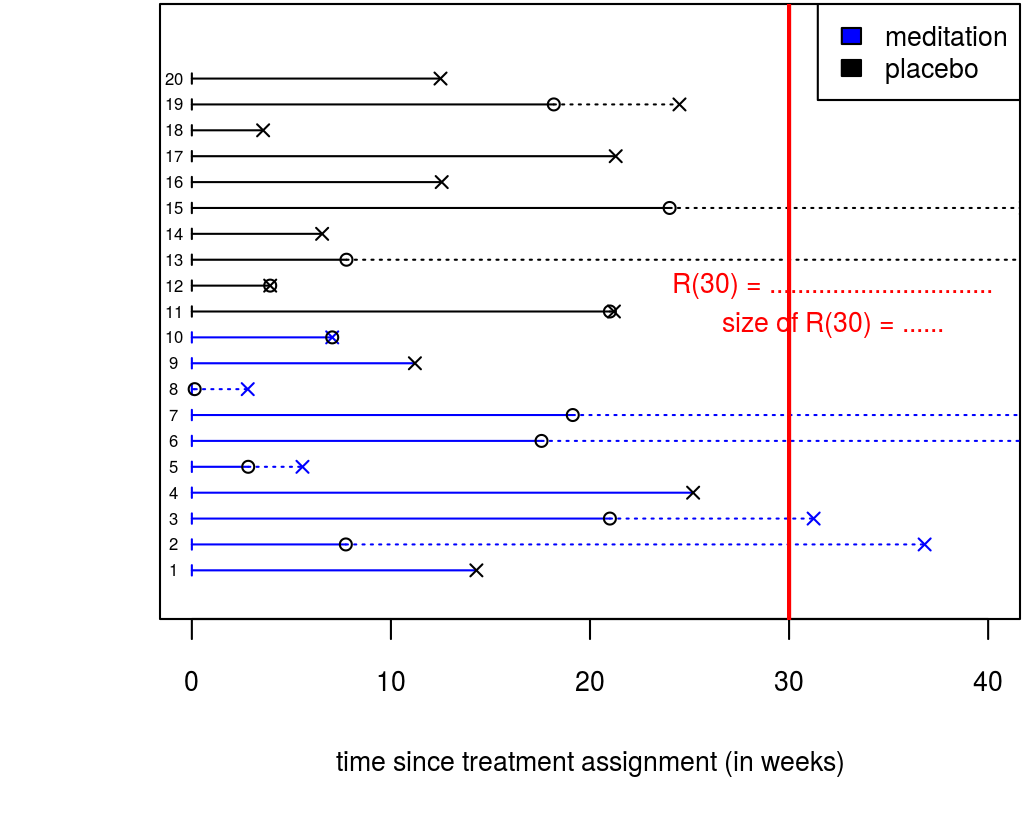
\includegraphics[height=0.8\textheight]{figs/risk_set_movie_6.png}
\end{center}
\end{frame}

\begin{frame}
\frametitle{Characteristics of survival data}
\begin{center}
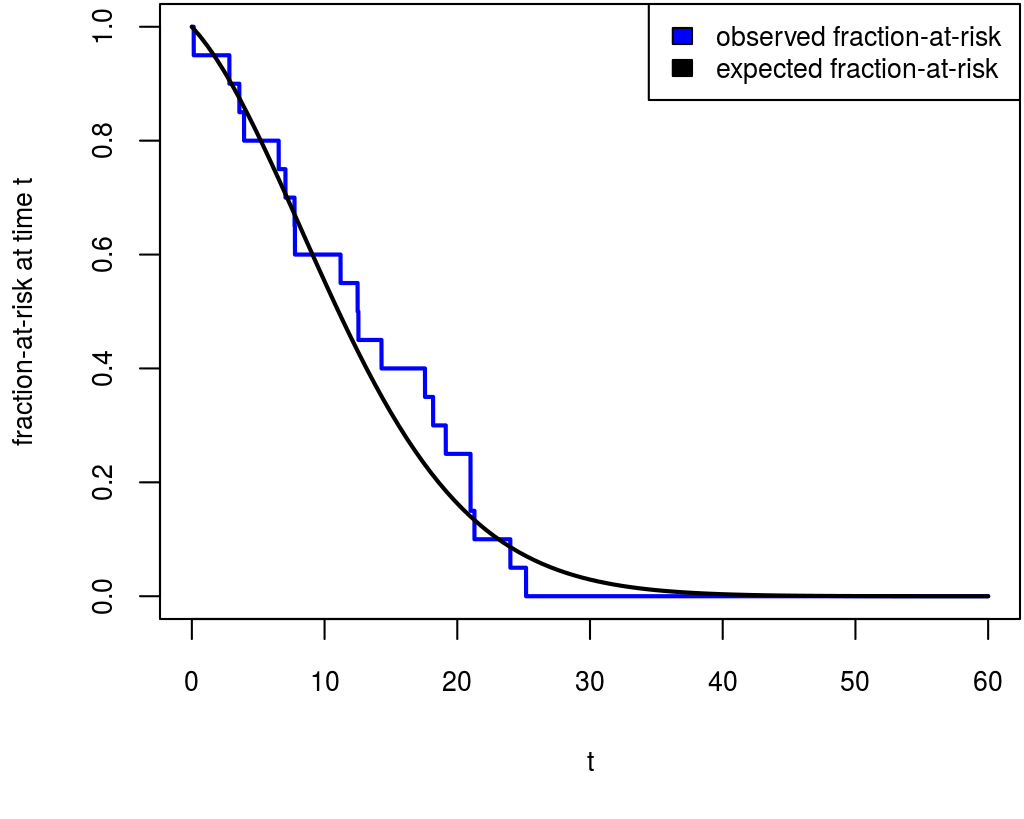
\includegraphics[height=0.8\textheight]{figs/risk_set.png}
\end{center}
\end{frame}
% uninformative censoring, with examples (from Anna)

\begin{frame}
\frametitle{Characteristics of survival data}
The assumption of \textbf{independent (or uninformative) censoring} is \textcolor{red}{critical} to the vast majority of methods available in survival analysis.

A participant's \textbf{time-to-event} and potential \textbf{censoring time} should be \textbf{independent} of one another.

What does that mean? \pause \textit{Individuals in the risk set at time $t$ must be \textbf{similar} to members of the target population who haven't experienced their first severe panic attack by time $t$.}

When is this reasonable? \vspace{-0.3cm}
\begin{itemize}
\item Participants are censored because the study ended? \pause \textcolor{blue}{Yes!}
\item Participants exited the study because their panic disorder became disabling? \pause \textcolor{red}{No!}
\item Participants exited the study because their panic disorder dissipated? \pause \textcolor{red}{No!}
\end{itemize}
\end{frame}

% key quantities: density function, survival function, hazard function
\begin{frame}
\frametitle{Key quantities in survival analysis}
Suppose that $T$ is a continuous, time-to-event random variable (\textcolor{blue}{$T$ is our outcome of interest in survival analysis}).

The \textbf{survival function}, $S$, is defined as $S(t) := P(T > t)$:
\begin{itemize}
\item $S(t) = $ proportion of the population with a time-to-event greater than $t$
\item e.g.: if $S(20) = 0.37$, then approximately 37\% of the population will not experience a severe panic attack within the first 20 weeks
\item $S$ is \textcolor{red}{non-increasing}, starts at 1 [i.e., $S(0) = 1$] and ends at 0 [i.e., $S(\infty) = 0$]
\end{itemize}
\end{frame}

\begin{frame}
\frametitle{Key quantities in survival analysis}
\hspace*{-0.5cm}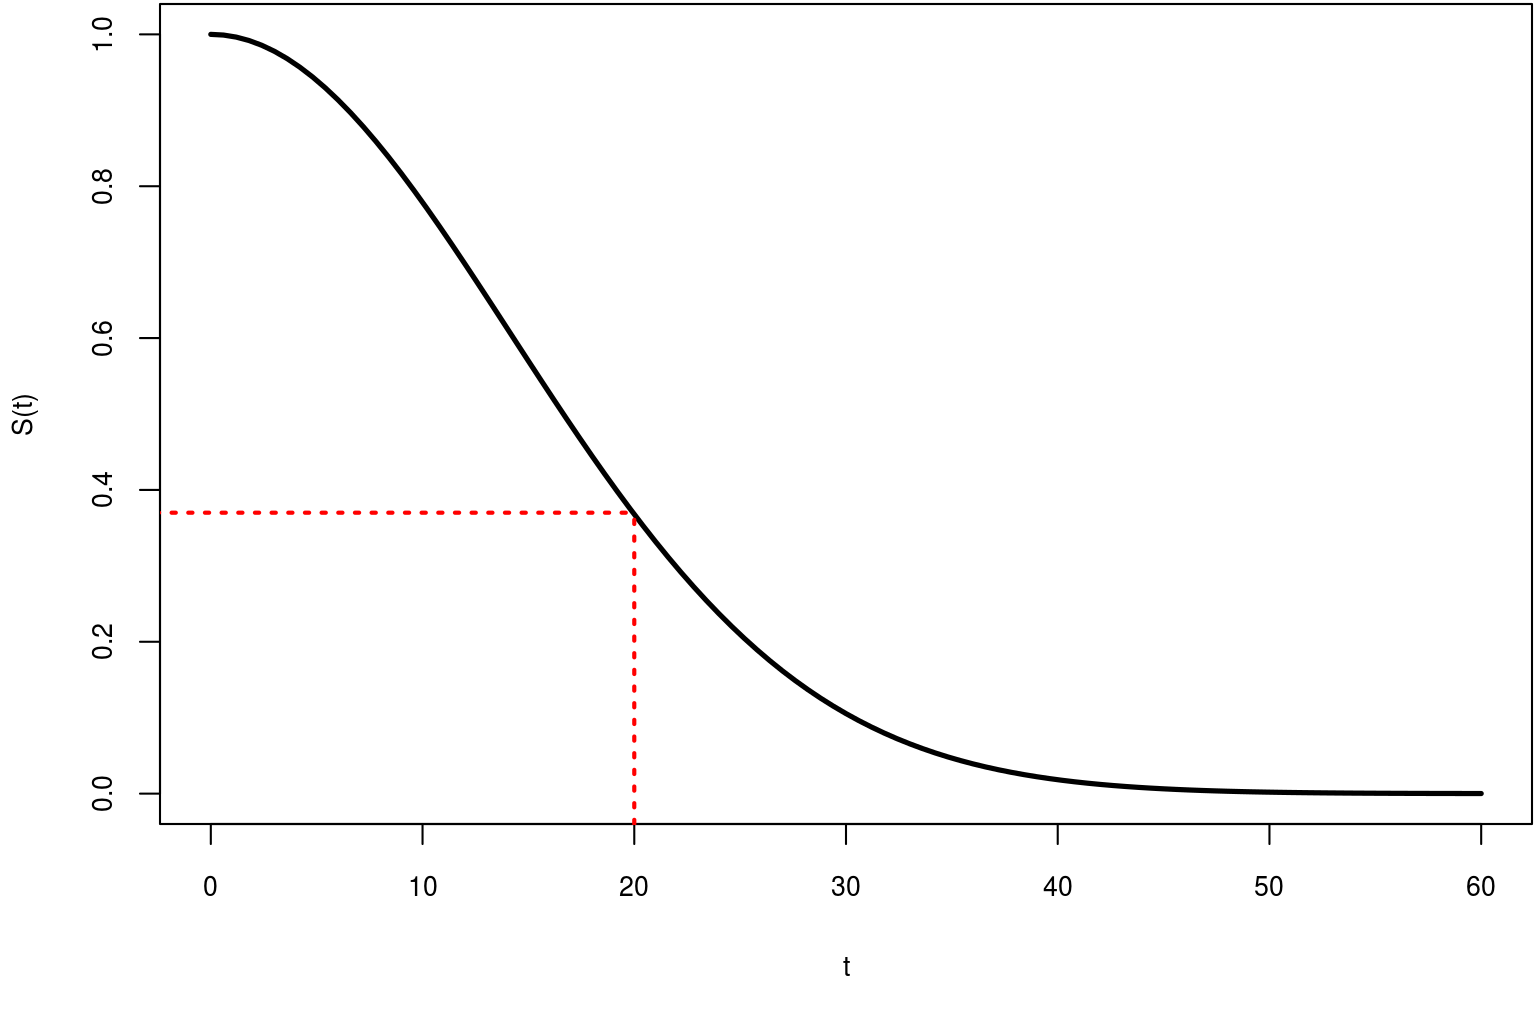
\includegraphics[height=0.8\textheight]{figs/survival_function.png}
\end{frame}

\begin{frame}
\frametitle{Key quantities in survival analysis}
The \textbf{hazard function} (or: hazard rate, failure rate) $h$ is \vspace{-0.2cm}
\begin{align*}
h(t) := & \ \lim_{\Delta t \to 0} \frac{P(t \leq T < t + \Delta t \mid T \geq t)}{\Delta t}.
\end{align*}\vspace{-0.8cm}
\begin{itemize}
\item $h(t) = $ instantaneous failure rate at $t$ given ``survival'' until $t$
\item $h(t)\Delta t$ approximates the probability that $T$ is in the interval $[t, t + \Delta t)$ given $T \geq t$
\item if $T$ corresponds to age at onset, $h(t)$ refers to the incidence rate at age $t$
\end{itemize}

The \textbf{cumulative hazard function} $H$ is given by $H(t) := \int_0^t h(u) du$.

\end{frame}

\begin{frame}
\frametitle{Key quantities in survival analysis}
\centering
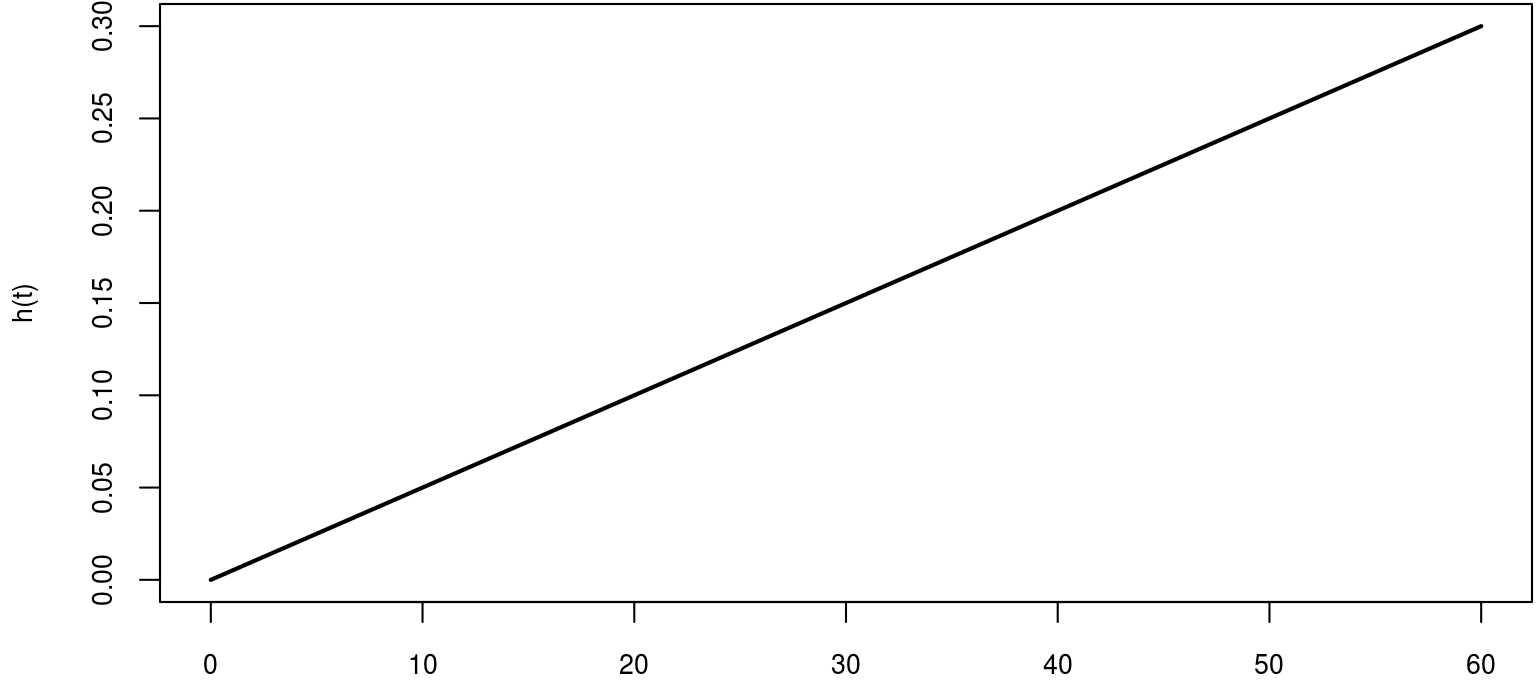
\includegraphics[height=0.4\textheight]{figs/hazard_function.png}

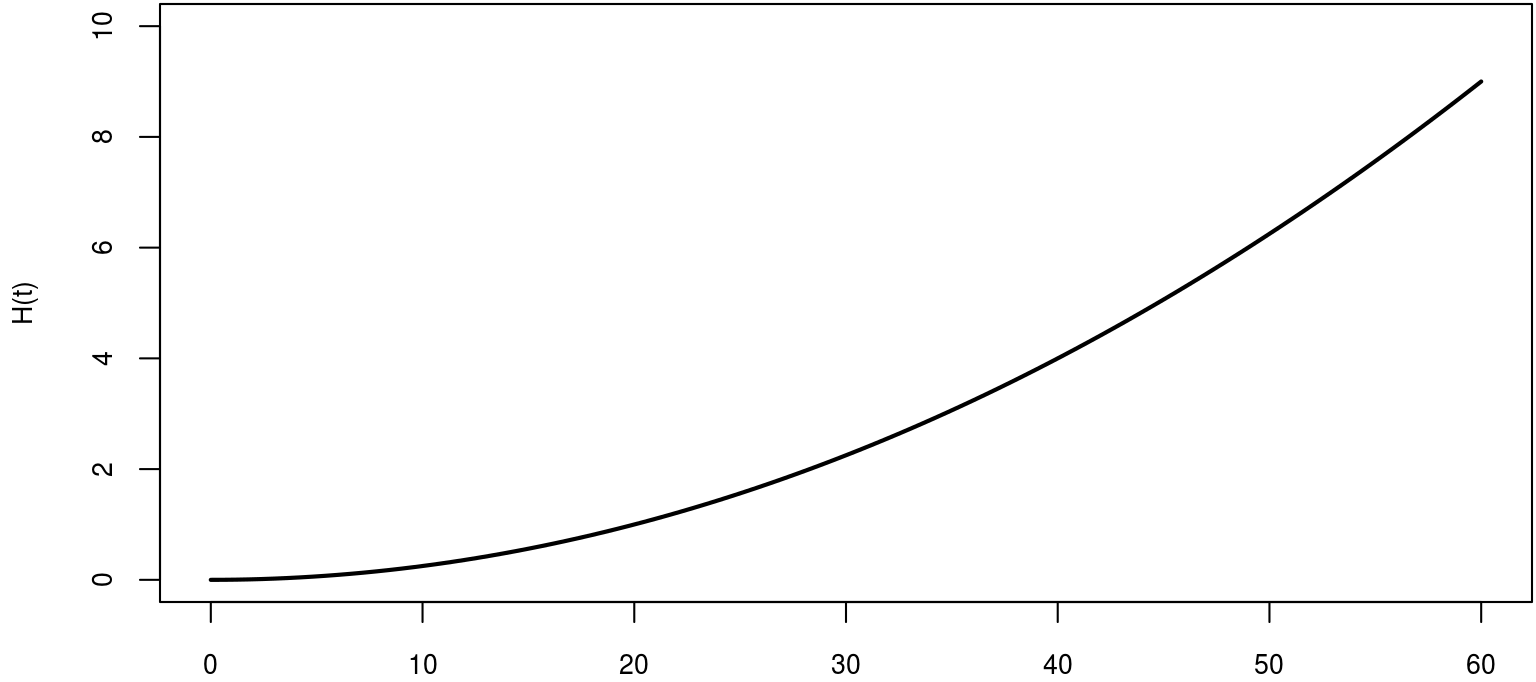
\includegraphics[height=0.4\textheight]{figs/cumulative_hazard_function.png}
\end{frame}

\begin{frame}
\frametitle{Key quantities in survival analysis}
Most methods in survival analysis focus on modeling and/or estimating either the \textcolor{cyan}{survival function} or the \textcolor{Aquamarine}{hazard rate}.

The hazard rate, while somewhat nonintuitive, has some desirable properties:
\begin{itemize}
\item its \textcolor{blue}{conditional interpretation} may be useful in many epidemiological applications
\item it can be \textcolor{blue}{easily estimated using right-censored data}
\end{itemize}
\end{frame}

\begin{frame}
\frametitle{Key quantities in survival analysis}
What shape do we expect the hazard function to have? \textcolor{red}{It depends...}
\begin{enumerate}[(a)]
\item survival from surgery until death due to complications
\item survival from onset of a progressive disease
\item the time before a radioactive atom disintegrates
\item an individual's total lifetime
\end{enumerate}
\begin{center}
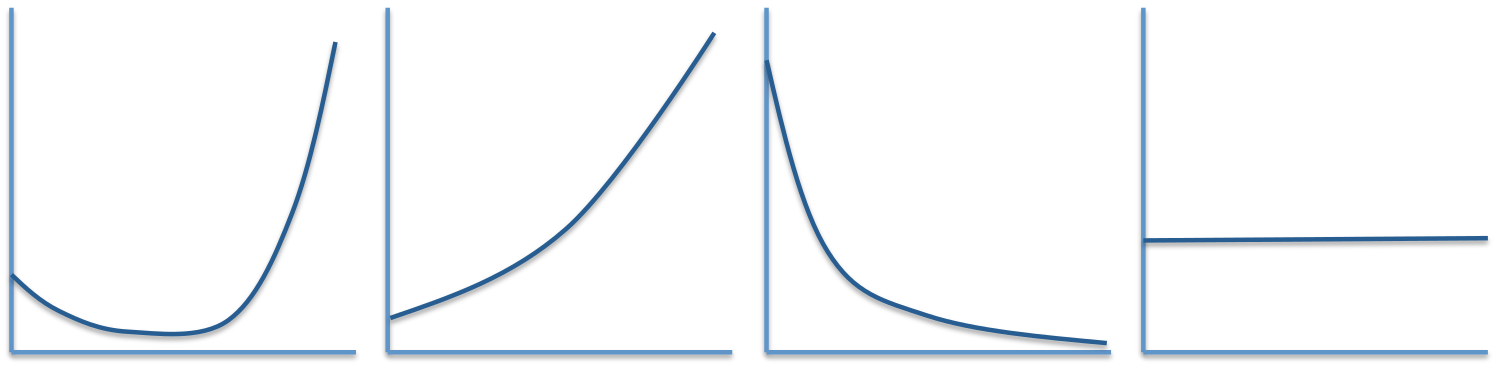
\includegraphics[width = 0.9\textwidth]{figs/hazard_examples.png}

\underline{\,\phantom{right}\,} \hspace{1.5cm} \underline{\,\phantom{right}\,} \hspace{1.5cm} \underline{\,\phantom{right}\,} \hspace{1.5cm} \underline{\,\phantom{right}\,}
\end{center}
\end{frame}

\section{Kaplan-Meier and the log rank test}
\begin{frame}
\frametitle{SECTION 2: KAPLAN-MEIER AND THE LOG RANK TEST}

So far, we have discussed challenges inherent to survival data and some quantities of interest. Now, we will discuss estimating these quantities from right-censored survival data.

For participant $i$, denote by $T_i$ \textbf{the time to event} and by $C_i$ \textbf{the censoring time}. We cannot observe both $T_i$ and $C_i$ -- instead, we observe a pair $(Y_i, \Delta_i)$, where \vspace{-0.3cm}
\begin{itemize}
\item $Y_i := \min(T_i, C_i)$ is the \textbf{observed follow-up time}
\item $\Delta_i = I(T_i \leq C_i)$ is the \textbf{event indicator} [where $I(x = 1)$ is 1 if $x = 1$ and zero otherwise]
\end{itemize}

For example, data represented as $\{7.5, 16.6+, 13.5+, 7.4, 14.2\}$ can now be written as
\[\{(7.5, \underline{\,\phantom{right}\,}), (16.6, \underline{\,\phantom{right}\,}), (13.5, \underline{\,\phantom{right}\,}), (7.4, \underline{\,\phantom{right}\,}), (14.2, \underline{\,\phantom{right}\,})\}.\]
\end{frame}

\begin{frame}
\frametitle{Estimation based on parametric models}

Our goal is generally to \textbf{describe the distribution of} $T$ or some summary of it, and to perform statistical inference to determine if survival differs based on a predictor of interest.

We could, for example, hypothesize that the distribution of $T$ is in a known \textbf{parametric model}, where once we know a parameter (e.g., the mean, standard deviation) we know the whole distribution of $T$.

\end{frame}

\begin{frame}
\frametitle{Estimation based on parametric models}

A variety of parametric families exist, but in survival analysis, the more popular ones are
\begin{itemize}
\item the exponential distribution
\item the Weibull distribution
\item the gamma distribution
\end{itemize}

Each parametric family has characteristics that may or may not make it suitable for the intended application.

However, use of a parametric model comes with a serious risk: \textbf{if the model is misspecified}, the validity of \textbf{our scientific conclusions may be compromised}.
\end{frame}

\begin{frame}
\frametitle{Nonparametric estimation of a survival function}

Suppose we focus on \textbf{estimating the survival probability} $S(t) = P(T > t)$ at time $t$.

If we observed actual survival times $T_1, T_2, \dots, T_n$, we could take
\begin{align*}
\frac{1}{n}\sum_{i=1}^n I(T_i \geq t)
\end{align*}
as an estimator of $S(t)$. This is a \textbf{nonparametric} estimator; we do not have to postulate a parametric model for the true survival distribution.

Can we use this estimator in practice? \pause No, since \textcolor{red}{we do not see $T_i$ for participants who are censored}!
\end{frame}

\begin{frame}
\frametitle{Nonparametric estimation of a survival function}

{\small Denote by $u_1 < u_2 < \dots < u_m$ the observed ordered, distinct times. Also, denote: \vspace{-1cm}

\begin{align*}
d_k = & \ \text{\# of events having occurred at time $u_k$} \\
n_k = & \ \text{\# of individuals at risk at time $u_k$}
\end{align*}
\vspace{-0.5cm}
Suppose the data consist of $\{4, 5, 5+, 8, 12+, 13, 18+, 23, 23, 30\}$.

\begin{center}
\begin{tabular}{|c|c|c|}
\hline
time $u_k$ & $d_k$ & $n_k$ \\
\hline
4 & 1 & 10 \\
5 & 1 & 9 \\
8 & 1 & 7 \\
12 & 0 & 6 \\
13 & 1 & 5 \\
18 & 0 & 4 \\
23 & 2 & 3 \\
30 & 1 & 1 \\
\hline
\end{tabular}
\end{center}
}
\end{frame}

\begin{frame}
\frametitle{Nonparametric estimation of a survival function}

{\small Suppose the data consist of $\{4, 5, 5+, 8, 12+, 13, 18+, 23, 23, 30\}$.}

\begin{center}
\begin{tabular}{|c|c|c|}
\hline
time $u_k$ & $d_k$ & $n_k$ \\
\hline
4 & 1 & 10 \\
5 & 1 & 9 \\
8 & 1 & 7 \\
12 & 0 & 6 \\
13 & 1 & 5 \\
18 & 0 & 4 \\
23 & 2 & 3 \\
30 & 1 & 1 \\
\hline
\end{tabular}
\end{center}

Is $m$ the number of events in the sample? \underline{\;\;\phantom{right}\;\;}

When does $m = n$? \underline{\;\;\phantom{right}\;\;}
\end{frame}

\begin{frame}
\frametitle{Nonparametric estimation of a survival function}

% here, do the probability estimates to walk up to KM (Marco slide 33)
\end{frame}

\begin{frame}
\frametitle{Nonparametric estimation of a survival function}

% Kaplan-Meier (Marco slide 34)
\end{frame}

\begin{frame}
\frametitle{Nonparametric estimation of a survival function}

% KM for this example (Marco 36)
\end{frame}

\begin{frame}
\frametitle{Nonparametric estimation of a survival function}

% picture (Marco 37)
\end{frame}

\begin{frame}
\frametitle{Nonparametric estimation of a survival function}

% standard error, CI (no formulas, just that they exist)
\end{frame}

\begin{frame}
\frametitle{Nonparametric estimation of a survival function}

% for this example (Marco, 39)
\end{frame}

\begin{frame}
\frametitle{Nonparametric estimation of a survival function}

% KM in a data analysis (time to death in inflamm)
\end{frame}


\begin{frame}
\frametitle{Nonparametric estimation of a survival function}

% mean, restricted mean, median (Marco, 63--70)
\end{frame}

\begin{frame}
\frametitle{Nonparametric estimation of a survival function}

% log-rank test (Marco 85--103)
\end{frame}

% motivate regression modeling

\begin{comment}
\section{Semiparametric estimation and inference}
\begin{frame}
\frametitle{SECTION 3: COX PROPORTIONAL HAZARDS REGRESSION}
\end{frame}

% cox ph regression, assumptions
\section{Summary}
\begin{frame}
\frametitle{SECTION 4: SUMMARY}
\end{frame}
% different ways to look at survival data
\end{comment}
\end{document}